\documentclass[11pt, a4paper]{article}
%\usepackage[utf8]{inputenc} % Umlaute moussen nicht maskiert werden
\usepackage{fontspec} % Umlaute im eps sind nicht zusammengesetzt
\usepackage{lmodern} % Vektor-Schriftart
\usepackage{ngerman} % Deutsche Silbentrennung (texlive-german und texlive-hyphen-german)
\usepackage{graphicx} % Einbinden von Grafiken / SVG-Dateien moussen zuvor als eps exportiert werden
\usepackage{url} % Four URLs in der Bibliographie
\usepackage{amstext} % Four nichtkursiven Text in Formeln
\usepackage{listings}
\usepackage[dvipsnames]{xcolor}
\lstset{
	numbers= left,
	language=C++,
	keywordstyle=\color{Blue},
	stringstyle=\color{Orange},
	commentstyle=\color{OliveGreen},
	breaklines=true,
	extendedchars=true,
	basicstyle=\footnotesize\ttfamily,
	tabsize=2,
	frame=single,
	rulecolor=\color{black},
	captionpos=b}
\lstset{literate={-}{{-\allowbreak}}{1} }
\usepackage{etoolbox}% http://ctan.org/pkg/etoolbox
\makeatletter
\patchcmd{\lst@GLI@}% <command>
{\def\lst@firstline{#1\relax}}% <search>
{\def\lst@firstline{#1\relax}\def\lst@firstnumber{#1\relax}}% <replace>
{\typeout{listings firstnumber=firstline}}% <success>
{\typeout{listings firstnumber not set}}% <failure>
\makeatother
\newcommand{\code}{\texttt}
\usepackage{textcomp}
\usepackage{gensymb}
\usepackage{float}
\usepackage{csquotes}
\usepackage{amsmath}
\usepackage{microtype}
\date{\today}
\begin{document}
\begin{center}
{\Huge Hochschule Darmstadt} \\
\vspace{0.5cm}
Lehrveranstaltung: Simulation von Robotersystemen \\
Prof. Dr. Thomas Horsch \\
Robotermodellierung und kinematische Transformationen\\
Datum: 29.4.2016 und 13.5.2016 \\
\vfill
\renewcommand{\arraystretch}{2}
	\begin{tabular}{| l | l |}
	\hline
	Name & Matrikelnummer \\ \hline
	Fabian Alexander Wilms & 735162 \\ \hline
	\end{tabular} \\
\vspace{0.5cm}
Studiengang: Mechatronik \\
Abgabedatum: 20.5.2016 \\
\vspace{0.5cm}
\begin{tabular}{| l | p{5cm} |}
	\hline
	Testat & \\ \hline
\end{tabular}
\renewcommand{\arraystretch}{1}
\end{center}
\newpage
\tableofcontents
\newpage
\section{Stabmodell}
Der erste Schritt auf dem Weg zu einer realistischen Simulation des Roboters Kuka KR3 in EasyRob ist das Stabmodell. Dafür müssen die Transformationsmatrizen zwischen den einzelnen Gelenkkoordinatensystemen aufgestellt werden. Anschließend kann die kinematische Struktur in EasyRob via \enquote{Robotics > cRobot Kinematics > Kinematics Data} eingegeben werden. Es muss die Anzahl aktiver Gelenke angegeben werden, ob es sich jeweils um ein Rotations- oder Translationsgelenk handelt und auf welche Achse sich die Gelenkvariable bezieht. Schließlich werden die Rotationen und Translationen zwischen den Koordinatensystemen eingegeben. Das Ergebnis ist das folgende Stabmodell:
\begin{figure}[H]
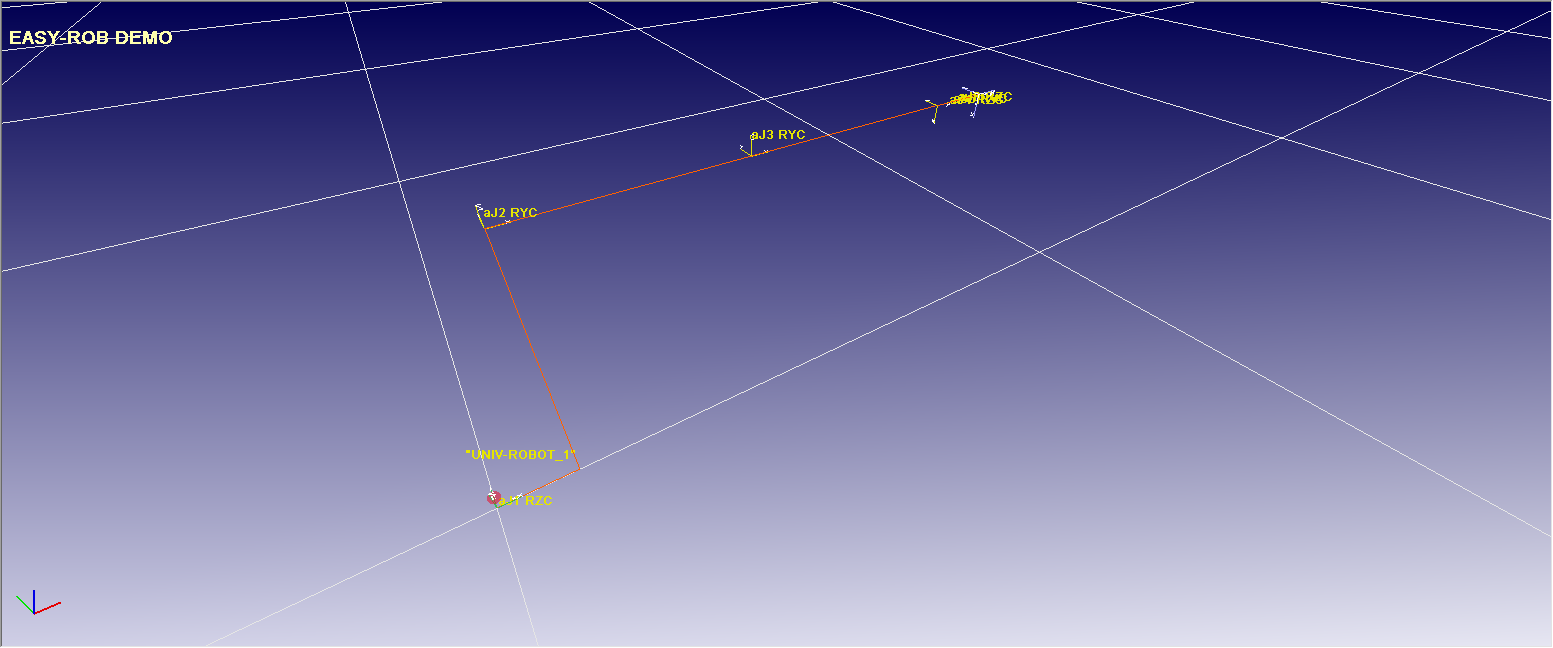
\includegraphics[width=\textwidth]{../Bilder/Aufgabe-1-Stabmodell-Demo.png}
\caption{Stabmodell}
\end{figure}
Dieses wird vor dem nächsten Schritt auf Richtigkeit überprüft. Dazu werden in EasyRob verschiedene Gelenkwinkel angefahren und die Rotationen mit dem Stabmodell in den Versuchsunterlagen abgeglichen.
\section{Realistisches Modell}
Damit das Modell auch optisch einem realen KR3 ähnelt, können 3D-Körper zum Stabmodell hinzugefügt werden. Polygonmodelle werden an die einzelnen Armteile angeheftet und ermöglichen es somit, Kollisionen leichter zu erkennen. Die Darstellung des zugrundeliegenden Stabmodells lässt sich über \enquote{View > Coorsys > Show Robot Coorsys} deaktivieren. Die Polygonmodelle liegen als einzelne Dateien im IGP Format vor. Das Fenster zum Anheften von CAD-Objekten öffnet man via \enquote{3D-CAD > Open 3D-CAD Window}. Dort muss man die Robot Group auswählen, damit die Objekte am Roboter fixiert werden. Über \enquote{Create Import} lassen sich IGP Teile importieren. Geschieht dies in der richtigen Reihenfolge von Armteil 0 bis Armteil 6 und mit dem Stabmodell in der Nullposition, so werden die Modelle automatisch an den korrekten Positionen eingefügt. Über den Wert des Schlüssels \enquote{Attach to active Joint} lässt sich das jeweilige Gelenk festlegen, an dem es fixiert wird.
\begin{figure}[H]
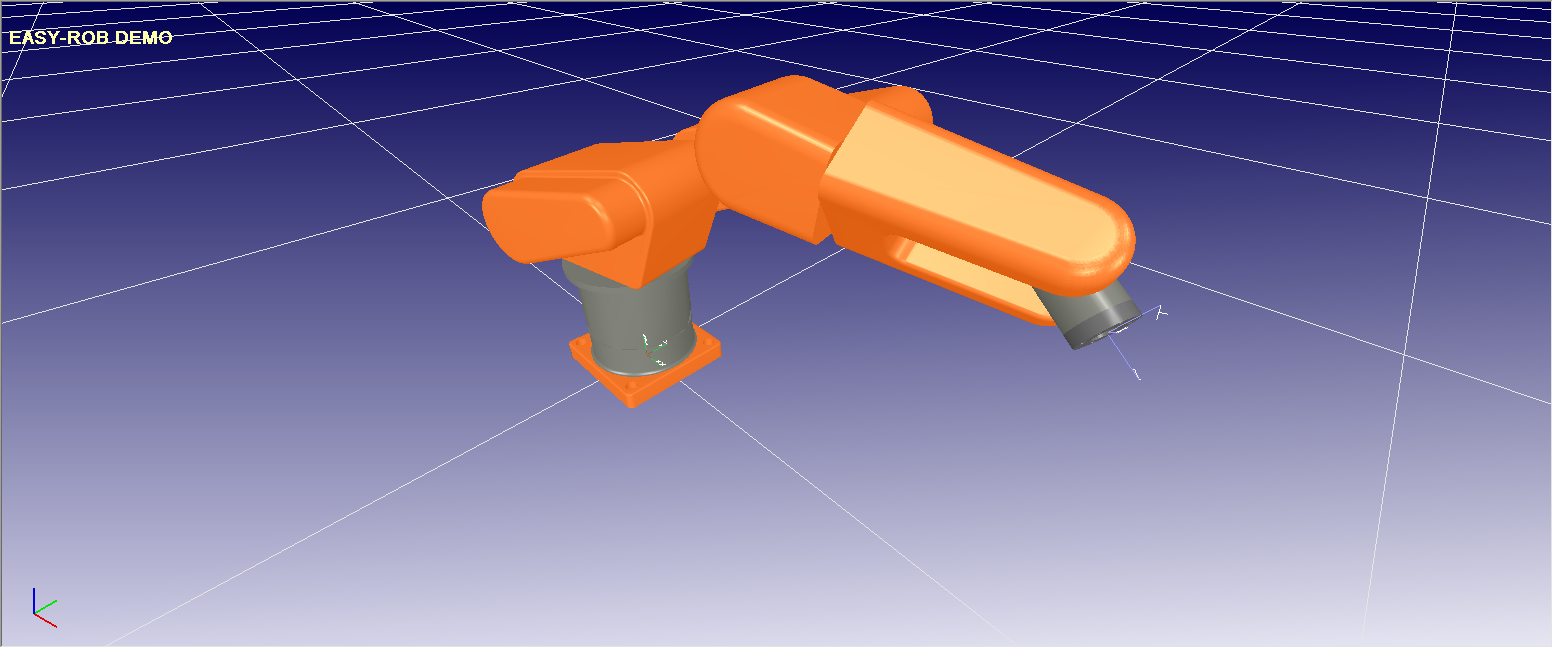
\includegraphics[width=\textwidth]{../Bilder/Aufgabe-2-Polygonmodell-Nicht-Home-Demo.png}
\caption{Realistisches Modell}
\end{figure}
\section{Vorwärtstransformation}
Mit der Vorwärtstransformation erhält man Position und Orientierung des TCP im kartesischen Koordinatensystem basierend auf den Gelenkstellungen. Zur Implementierung der Vorwärtstransformation in C++, unabhängig von EasyRob wurde die Vectmath-Bibliothek aus dem Microb-Projekt verwendet. Dieses wurde vom Unternehmen Hydro-Québec entwickelt. Vectmath stellt eine Reihe von Klassen bereit, welche für Berechnungen mit Matrizen benötigt werden. In einem ersten Schritt wird die kinematische Struktur des KR3 im Code dargestellt. Dazu dient das Array KR3[6] des Typs KinematicData mit 6 Feldern. Der Datentyp KinematicData beschreibt für jedes Gelenk den Typ und die jeweils drei Rotations- sowie Translationskomponenten der Transformation zum nächsten Koordinatensystem. Jedem Feld der Variablen KR3 werden mit einer Schleife jeweils die Werte für Typ, Translation und Rotation zugewiesen. Dafür werden zuerst 7 Arrays angelegt, je eines für jede Member-Variable, mit jeweils 6 Feldern, einem pro Gelenk.

\vspace{\baselineskip}
\centerline{\begin{tabular}{|c|c|c|c|c|c|c|c|c|} \hline
	Gelenk & Art & Achse & Trans X & Trans Y & Trans Z & Rot X & Rot Y & Rot Z \\ \hline
	1 & ROT & z & 100 & 265 & 270 & 0 & 0 & 0 \\ \hline
	2 & ROT & y & 0 & 0 & 0 & 0 & 0 & 0 \\ \hline
	3 & ROT & y & 350 & 0 & 0 & 0 & 75 & 0 \\ \hline
	4 & ROT & z & 0 & 0 & 0 & 0 & 0 & 0 \\ \hline
	5 & ROT & y & 0 & 0 & 90 & 0 & 0 & 0 \\ \hline
	6 & ROT & z & 0 & 0 & 0 & 0 & 0 & 0 \\ \hline
\end{tabular}}

\vspace{\baselineskip}
\lstinputlisting[firstline=49,lastline=95,caption={kinematische Struktur}]{../C++Projekt/Termin2u3/Termin2u3.cpp}

Das Ziel der Vorwärtstransformation ist es, aus den Gelenkwinkeln zu Position und Orientierung des Tool Center Point (TCP) in kartesischen Weltkoordinaten zu gelangen. Dazu muss das i-te Gelenk um den Wert der Gelenkvariablen $q_i$ um die Gelenkachse gedreht, bzw. auf ihr verschoben werden und anschließend die Transformation zum nächsten Gelenkkoordinatensystem durchgeführt werden. Dazu muss basierend auf dem Gelenktyp und dem Wert der Gelenkvariablen je Gelenk eine Transformationsmatrix erstellt werden und eine weitere, basierend auf den Werten, welche im Array KR3[] für jedes Gelenk gespeichert sind, mit der man Position und Orientierung des nächsten Gelenkkoordinatensystems erhält. Dabei muss darauf geachtet werden, dass die Winkelangaben der kinematischen Struktur und die Gelenkvariablen in Grad angegeben werden und daher in Radians umgerechnet werden müssen.

\lstinputlisting[firstline=126,lastline=170,caption={\code{ForwardKinematics()}}]{../C++Projekt/Termin2u3/Termin2u3.cpp}

Ein Aufruf der Funktion \code{ForwardKinematics()} mit den Gelenkwinkeln \code{axes(0.0, -142.65, 96.1763, 0.0, 51.4737, 0.0)} als Argument ergab folgende homogene Transformationsmatrix:

\begin{center}
	$T = \begin{bmatrix}
	-0.087156 & 0.000000 & 0.996195 & 149.999965 \\ 
	0.000000 & 1.000000 & 0.000000 & 0.000000 \\ 
	-0.996195 & 0.000000 & -0.087156 & 699.999891 \\ 
	0.000000 & 0.000000 & 0.000000 & 1.000000
	\end{bmatrix}$
\end{center}

Gibt man obige Gelenkwinkel in EasyRob ein und öffnet das Fenster mit der Ausgabe der Pose in kartesischen Weltkoordinaten via \enquote{View > Open Online Output Data}, so sieht man, dass die Werte mit den selbst errechneten übereinstimmen.

\begin{figure}[H]
	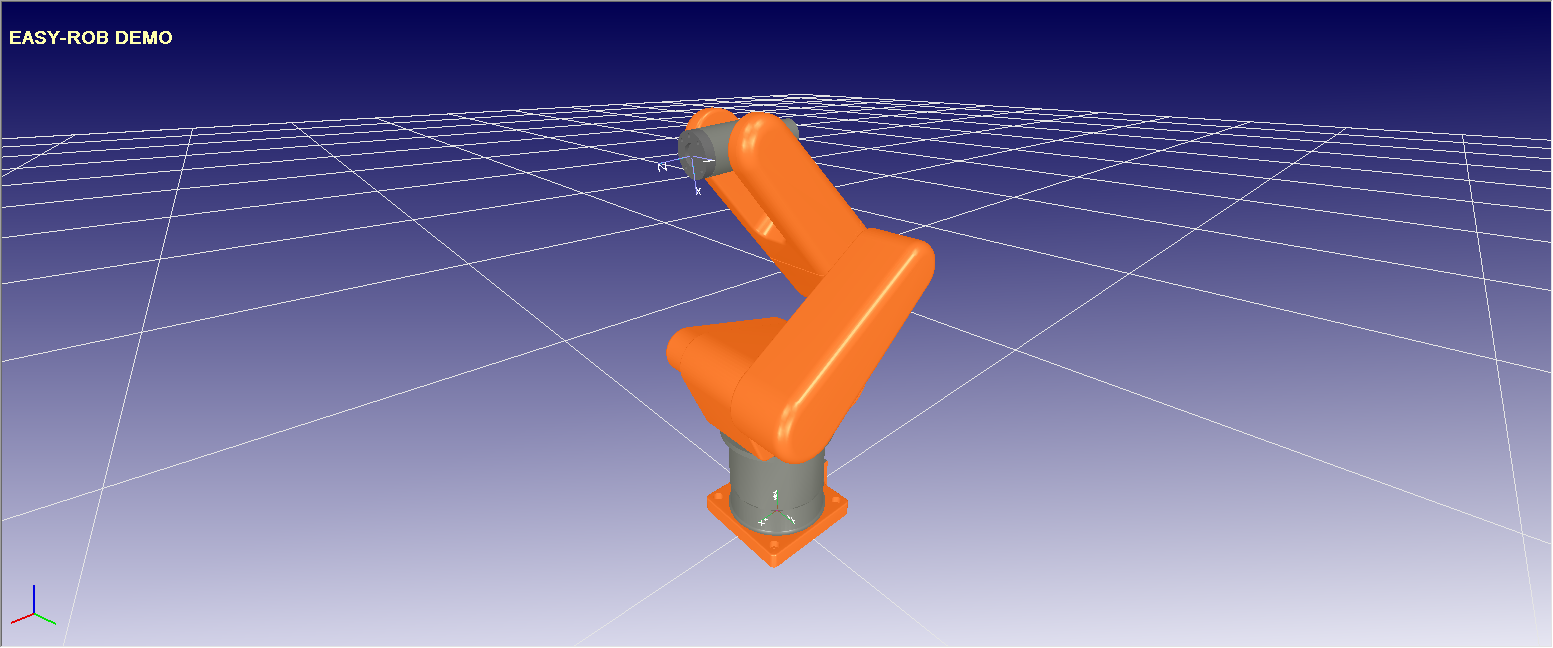
\includegraphics[width=\textwidth]{../Bilder/Aufgabe-3-VK.png}
	\caption{Pose in EasyRob}
\end{figure}
\begin{figure}[H]
	\center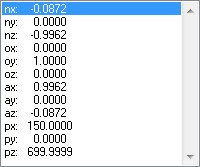
\includegraphics[width=0.5\textwidth]{../Bilder/Aufgabe-3-VK-Werte.png}
	\caption{Ergebnisse des obigen Algorithmus stimmen mit EasyRob überein}
\end{figure}

\section{Rückwärtstransformation}
Das Ziel der Rückwärtstransformation (inversen Kinematik) ist die Bestimmung der Gelenkwinkel bei gegebener Position und Orientierung des TCP in kartesischen Weltkoordinaten. Die inverse Kinematik kann geometrisch oder numerisch berechnet werden. Hier wurde die zweite Möglichkeit gewählt. Der erste Schritt der numerischen Berechnung der inversen Kinematik ist die Bestimmung der Jacobi-Matrix im Arbeitspunkt, welcher durch die Gelenkvariable \code{axes} gegeben ist. Dies linearisiert den Zusammenhang zwischen Gelenkvariablen und kartesischen Koordinaten in der Nähe des Arbeitspunktes.

\begin{eqnarray*}
	J(\underline{q}) \cdot \Delta \underline{q} &= \Delta \underline{x} \quad | \cdot J^{-1}(\underline{q}) \\
	\Delta \underline{q} &= J^{-1}(\underline{q}) \cdot \Delta \underline{x}
\end{eqnarray*} 

Spalte $i$ der Jacobi-Matrix besteht aus der numerisch nach der Gelenkvariablen $q_k$ differenzierten Spalte $i$ der Vorwärtstransformation. Die Berechnung der Jacobi-Matrix bei gegebener kinematischer Struktur und Gelenkwinkeln geschieht in der Funktion \code{ikNumDiff()}.

Zur Berechnung der numerischen Differentiation bildet man den Vorwärtsdifferenzenquotienten. Dazu wird zunächst die momentane kartesische Pose in einer Variablen vom Typ \code{Angle\_axis\_xyz} gespeichert. Dann werden nacheinander die einzelnen Gelenkvariablen um den Wert \code{delta} erhöht, damit eine zweite Vorwärtskinematik berechnet und daraus der Spaltenvektor der Differenzenquotienten gebildet. Die einzelnen Spalten werden nebeneinander gesetzt und bilden so eine Matrix der Dimension 6x6.

Die so bestimmte Jacobi-Matrix wird von der Funktion zurückgegeben.

\lstinputlisting[firstline=182,lastline=208,caption={\code{ikNumDiff()}}]{../C++Projekt/Termin2u3/Termin2u3.cpp}

Die oben erläuterte Funktion zur Bestimmung der Jacobi-Matrix im Arbeitspunkt wird innerhalb der Funktion \code{InverseKinematics()} aufgerufen. Zunächst wird die Jacobi-Matrix zum übergebenen Gelenkwinkelvektor bestimmt und dann invertiert. Die dazu benutzte Funktion \code{ikSVD()} ist robust gegenüber Rangdefekten, welche in der Nähe von singulären Stellungen auftreten können. Dann wird in einer Schleife \code{dq} mithilfe der invertierten Jacobi-Matrix und der kartesischen Differenz zwischen gewünschten und TCP-Koordinaten und den aus den aktuellen Gelenkstellungen berechneten aktuellen Koordinaten bestimmt.

Da jedoch alle Gelenke rotatorisch sind, erreicht man nach einem Durchlauf der Schleife meist nicht die gewünschten TCP-Koordinaten. Ob die neuen Koordinaten nah genug an den gewünschten sind, wird mithilfe einer Größe $\epsilon$ bestimmt. Sind der erreichte Punkt nah genug am Ziel und die benötigten Gelenkänderungen ebenfalls klein genug, so wird die Schleife abgebrochen und die neuen Gelenkvariablen werden von der Funktion zurückgegeben. Sind die Bedingungen noch nicht erfüllt, so wird eine neue Jacobi-Matrix um den neuen Punkt bestimmt und die Schleife wird ein weiteres mal durchlaufen. Um Endlosschleifen bei unerreichbaren TCP-Positionen oder Sprüngen der Gelenkvariablen aufgrund von numerischen Fehlern zu vermeiden, bricht die Schleife nach spätestens 100 Durchläufen ab.

\lstinputlisting[firstline=210,lastline=252,caption = {\code{InverseKinematics()}}]{../C++Projekt/Termin2u3/Termin2u3.cpp}

\section{Linearbewegung}
Die Funktion \code{IpoLin()} erzeugt aus einer gegebenen  kinematischen Struktur, Start- und Endposition in Gelenkkoordinaten und der gewünschten Anzahl an Interpolationsschritten ein EasyRob-Programm, dass eine Linearbahn zwischen beiden Positionen fährt.

Dazu werden aus den gewünschten Gelenkwinkeln für Start- und Endposition mit der Vorwärtskinematik die kartesischen Koordinaten des TCP berechnet. Zwischen beiden Punkten werden $n$ Punkte linear interpoliert. $n$ wird als Argument beim Aufruf von \code{IpoLin()} übergeben. Für jeden dieser Punkte werden die Gelenkstellungen mittels der inversen Kinematik berechnet.

\lstinputlisting[firstline=108,lastline=115,caption = {\code{IpoLin()}}]{../C++Projekt/Termin2u3/Termin2u3.cpp}

Das erzeugte EasyRob-Programm sieht wie folgt aus:

\lstinputlisting[firstline=1,lastline=3,caption = {Anfang kr3.prg}]{../C++Projekt/Termin2u3/kr3.prg}

\lstinputlisting[firstline=99,lastline=101,caption = {Ende kr3.prg}]{../C++Projekt/Termin2u3/kr3.prg}

\begin{figure}[H]
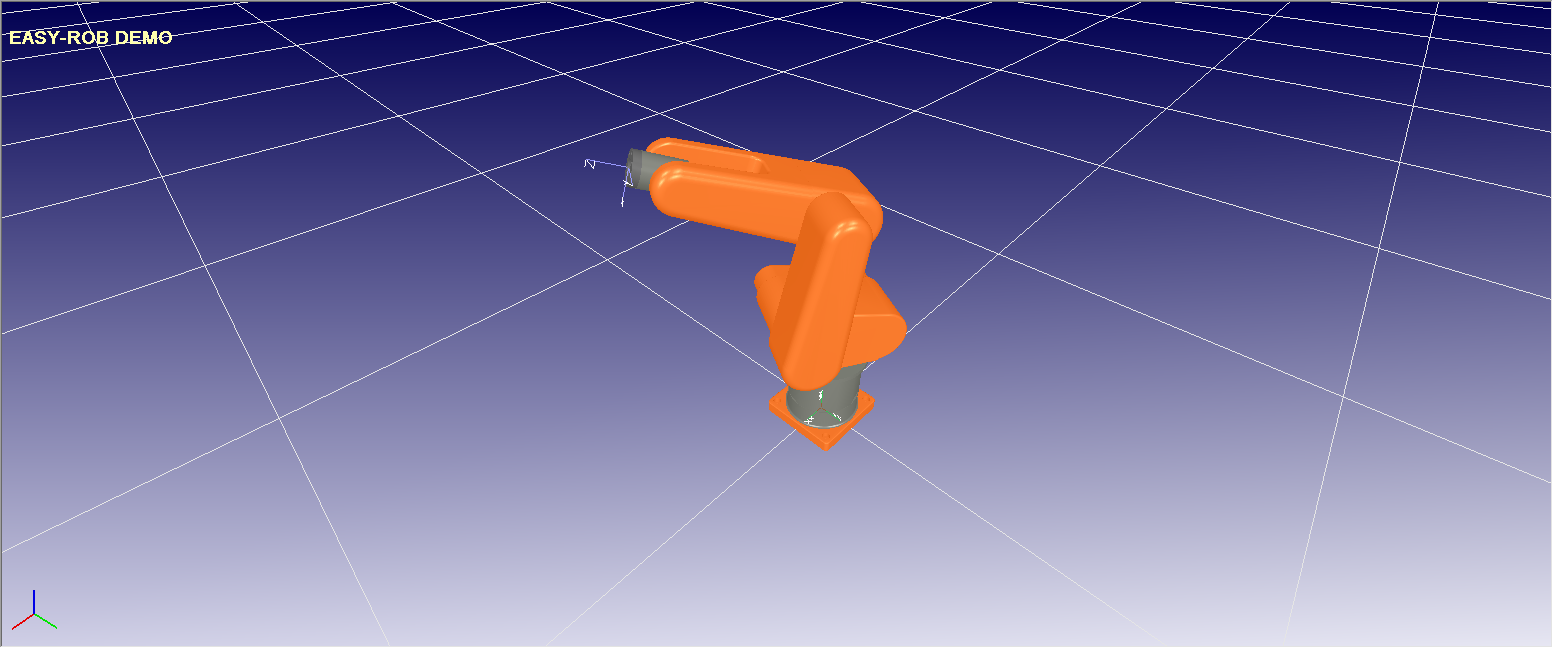
\includegraphics[width=\textwidth]{../Bilder/Aufgabe-5-IK-Startpos-Demo.png}
\caption{Startposition}
\end{figure}
Die Linearbahn des TCP wurde mithilfe der Funktion \enquote{View > TCP Trace > TCP Trace ON/OFF} sichtbar gemacht.
\begin{figure}[H]
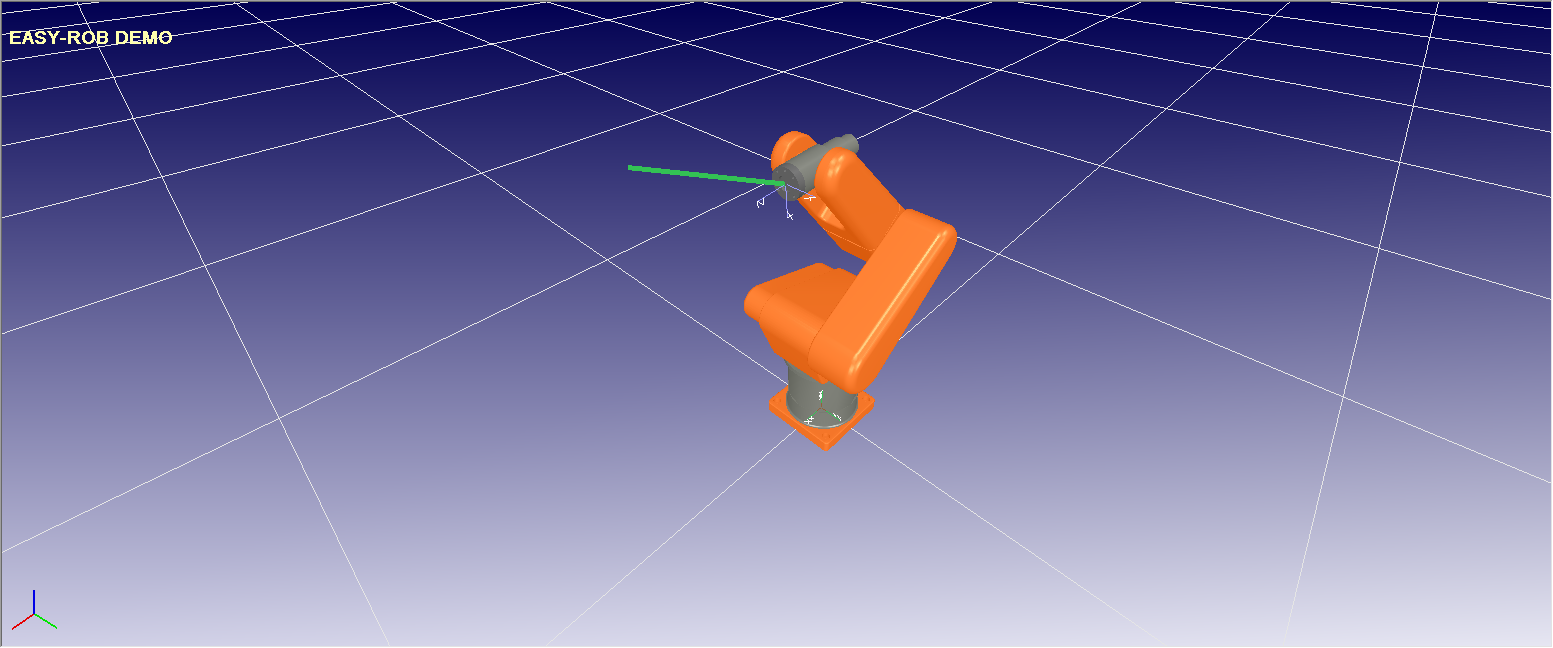
\includegraphics[width=\textwidth]{../Bilder/Aufgabe-5-IK-Endpos-Demo.png}
\caption{Endposition}
\end{figure}

Beim ersten Versuch, eine Linearbahn zu fahren trat ein Fehler auf: Der Arm machte einen relativen großen Sprung und schien sich danach nicht mehr zu bewegen. Grund war, dass als Ausgangsposition die Nullposition gewählt worden war. Da dann die Gelenkachsen 4 und 6 in einer Flucht liegen verliert man einen Freiheitsgrad: man befindet sich in einer Randsingularität. Eine Lösung des Problems wäre es, einen Algorithmus zu schreiben, der Singularitäten anhand der resultierenden äußerst großen Gelenkwinkeln erkennt und dann einzelne Gelenke minimal zu verfahren, um die Singularität zu eliminieren.
\lstinputlisting[firstline=1,lastline=3,caption = {Anfang kr3-singularitaet.prg}]{../C++Projekt/Termin2u3/kr3-singularitaet.prg}
\lstinputlisting[firstline=99,lastline=101,caption = {Ende kr3-singularitaet.prg}]{../C++Projekt/Termin2u3/kr3-singularitaet.prg}
\end{document}